\documentclass[aspectratio=169, 11pt]{beamer}

% ──────────────────────────────────────────────
% Theme & Styling
% ──────────────────────────────────────────────
\usetheme{Madrid}
\usecolortheme{seahorse}
\setbeamertemplate{navigation symbols}{}
\setbeamertemplate{footline}[frame number]
\setbeamertemplate{itemize items}[circle]
\setbeamertemplate{enumerate items}[default]

% ──────────────────────────────────────────────
% Packages
% ──────────────────────────────────────────────
\usepackage{graphicx}
\usepackage{tikz}
\usetikzlibrary{arrows.meta, positioning, shapes.geometric, calc, decorations.pathmorphing, fit}
\usepackage{amsmath, amssymb}
\usepackage{booktabs}
\usepackage{listings}
\usepackage{xcolor}
\usepackage{hyperref}
\usepackage{multicol}

% ──────────────────────────────────────────────
% Custom Colors
% ──────────────────────────────────────────────
\definecolor{tangleblue}{RGB}{41, 98, 255}
\definecolor{tangleteal}{RGB}{0, 150, 136}
\definecolor{tangleorange}{RGB}{255, 111, 0}
\definecolor{tanglered}{RGB}{211, 47, 47}
\definecolor{tanglegray}{RGB}{96, 96, 96}
\definecolor{lightbg}{RGB}{245, 245, 250}

% ──────────────────────────────────────────────
% Listings Style
% ──────────────────────────────────────────────
\lstset{
  basicstyle=\ttfamily\scriptsize,
  keywordstyle=\color{tangleblue}\bfseries,
  commentstyle=\color{tanglegray}\itshape,
  stringstyle=\color{tangleteal},
  backgroundcolor=\color{lightbg},
  frame=single,
  framerule=0.5pt,
  rulecolor=\color{tanglegray!30},
  breaklines=true,
  showstringspaces=false,
  tabsize=2
}

% ──────────────────────────────────────────────
% Title Information
% ──────────────────────────────────────────────
\title[TipSelection]{\textbf{TipSelection: Architecture \& Design}}
\subtitle{A Distributed Tangle Simulator with MCMC-Based Tip Selection}
\author{Anirudh Saikrishnan}
\date{\today}

\begin{document}

% ══════════════════════════════════════════════
% TITLE SLIDE
% ══════════════════════════════════════════════
\begin{frame}
  \titlepage
\end{frame}

% ══════════════════════════════════════════════
% OUTLINE
% ══════════════════════════════════════════════
\begin{frame}{Outline}
  \tableofcontents
\end{frame}

% ══════════════════════════════════════════════
\section{Project Overview}
% ══════════════════════════════════════════════

\begin{frame}{What Is This Project?}
  \begin{block}{Goal}
    Simulate the \textbf{IOTA Tangle}---a DAG-based distributed ledger---and study the behavior of different \textbf{tip selection algorithms} in a multi-node network setting.
  \end{block}

  \vspace{0.3cm}
  \textbf{Two independent implementations:}
  \begin{enumerate}
    \item \texttt{tangle-distributed} --- True multi-process simulation over TCP
    \item \texttt{tangle-sim} --- Single-process async cooperative simulation
  \end{enumerate}

  \vspace{0.3cm}
  \textbf{Based on two research papers:}
  \begin{itemize}
    \item \v{Z}ivi\'{c} et al.\ (TELFOR 2019): \emph{``DAG as Tangle: an IoT Alternative to Blockchains''}
    \item Ferraro, King \& Shorten (IEEE 2020): \emph{``On the Stability of Unverified Transactions in a DAG-based Distributed Ledger''}
  \end{itemize}
\end{frame}

% ══════════════════════════════════════════════
\section{Libraries \& Dependencies}
% ══════════════════════════════════════════════

\begin{frame}{Libraries \& Dependencies}
  \begin{columns}[T]
    \begin{column}{0.48\textwidth}
      \textbf{\texttt{tangle-distributed}}
      \begin{itemize}
        \item \texttt{asyncio} (stdlib) --- event loop, TCP servers/clients
        \item \texttt{subprocess} (stdlib) --- process spawning
        \item \texttt{matplotlib} $\geq$ 3.7 --- visualization
        \item \texttt{numpy} $\geq$ 1.24 --- statistics \& arrays
        \item \texttt{pyyaml} $\geq$ 6.0 --- YAML config parsing
        \item No external networking library
      \end{itemize}
    \end{column}
    \begin{column}{0.48\textwidth}
      \textbf{\texttt{tangle-sim}}
      \begin{itemize}
        \item \texttt{asyncio} (stdlib) --- cooperative tasks
        \item \texttt{pyzmq} $\geq$ 25.0 --- ZeroMQ (optional)
        \item \texttt{networkx} $\geq$ 3.0 --- graph algorithms
        \item \texttt{matplotlib} $\geq$ 3.7 --- visualization
        \item \texttt{numpy} $\geq$ 1.24 --- statistics
        \item \texttt{pyyaml} $\geq$ 6.0 --- config
        \item \texttt{rich} $\geq$ 13.0 --- terminal formatting
      \end{itemize}
    \end{column}
  \end{columns}

  \vspace{0.4cm}
  \begin{center}
    \small Python $\geq$ 3.10 required \quad$\bullet$\quad No external database---all state held in memory
  \end{center}
\end{frame}

% ══════════════════════════════════════════════
\section{Project Structure}
% ══════════════════════════════════════════════

\begin{frame}{High-Level Directory Layout}
  \begin{columns}[T]
    \begin{column}{0.48\textwidth}
      \textbf{\texttt{tangle-distributed/}}
      \begin{itemize}
        \item \texttt{core/} --- Transaction, Tangle DAG, Tip Selection, PoW, Validation
        \item \texttt{network/} --- Wire protocol, Peer connections, Latency model
        \item \texttt{node/} --- Autonomous node process logic
        \item \texttt{simulation/} --- Launcher (process spawner), Aggregator
        \item \texttt{viz/} --- Matplotlib dashboard
        \item \texttt{config/} --- YAML scenarios
        \item \texttt{scripts/} --- Entry points
        \item \texttt{tests/} --- Unit \& integration tests
      \end{itemize}
    \end{column}
    \begin{column}{0.48\textwidth}
      \textbf{\texttt{tangle-sim/src/}}
      \begin{itemize}
        \item \texttt{core/} --- Transaction, Tangle DAG, PoW
        \item \texttt{consensus/} --- Abstract base + 3 selectors
        \item \texttt{network/} --- Node, Message, Transport, Gossip, Topology
        \item \texttt{simulation/} --- Engine, Scenario loader, Metrics
        \item \texttt{validation/} --- Consistency, Double-spend detection
        \item \texttt{visualization/} --- Tangle viz, Metrics dashboard
        \item \texttt{config/} --- YAML scenarios
        \item \texttt{scripts/} --- Entry points
        \item \texttt{tests/} --- Test suite
      \end{itemize}
    \end{column}
  \end{columns}
\end{frame}

% ══════════════════════════════════════════════
\section{Core Data Structures}
% ══════════════════════════════════════════════

\begin{frame}{The Transaction}
  \begin{block}{Fields}
    \begin{itemize}
      \item \texttt{tx\_id} (str) --- unique identifier (hash)
      \item \texttt{issuer} (str) --- node that created it
      \item \texttt{parents[]} (list[str]) --- IDs of $m$ approved transactions (DAG edges)
      \item \texttt{value} (float), \texttt{sender\_addr}, \texttt{receiver\_addr} --- transfer data
      \item \texttt{timestamp} (float), \texttt{nonce} (int) --- metadata \& PoW proof
      \item \texttt{status} $\in$ \{\textsc{Pending\_PoW}, \textsc{Attached}, \textsc{Confirmed}\}
      \item \texttt{cumulative\_weight} (int) --- number of direct + indirect approvers + 1
    \end{itemize}
  \end{block}

  \vspace{0.2cm}
  \textbf{Serialization:} \texttt{to\_dict()} / \texttt{from\_dict()} for JSON transport over the wire.

  \vspace{0.2cm}
  \textbf{Identity:} \texttt{\_\_hash\_\_} and \texttt{\_\_eq\_\_} based on \texttt{tx\_id} for set membership.
\end{frame}

\begin{frame}{The Tangle (DAG)}

  \begin{columns}[T]
    \begin{column}{0.55\textwidth}
      \textbf{Internal State:}
      \begin{itemize}
        \item \texttt{\_txs}: \texttt{dict[str, Transaction]} --- all transactions
        \item \texttt{\_children}: \texttt{dict[str, set[str]]} --- reverse adjacency (who approves whom)
        \item \texttt{\_tips}: \texttt{set[str]} --- leaf nodes (no approvers)
        \item \texttt{\_genesis\_id}: the single root transaction
      \end{itemize}

      \vspace{0.3cm}
      \textbf{Key Operations:}
      \begin{itemize}
        \item \texttt{attach(tx)} --- insert into DAG, propagate weight
        \item \texttt{free\_tips} --- tips with completed PoW
        \item \texttt{children\_of(id)} --- direct approvers
        \item \texttt{approval\_path(id)} --- BFS to all ancestors
        \item \texttt{edge\_list()} --- for visualization
      \end{itemize}
    \end{column}
    \begin{column}{0.42\textwidth}
      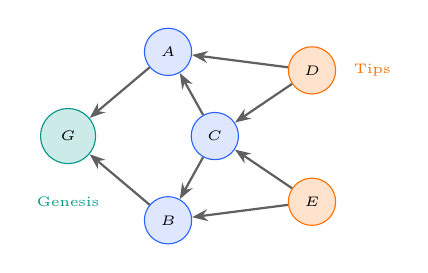
\begin{tikzpicture}[
        node distance=0.8cm and 1.0cm,
        tx/.style={circle, draw=tangleblue, fill=tangleblue!15, minimum size=0.6cm, font=\tiny\bfseries},
        tip/.style={circle, draw=tangleorange, fill=tangleorange!20, minimum size=0.6cm, font=\tiny\bfseries},
        gen/.style={circle, draw=tangleteal, fill=tangleteal!20, minimum size=0.7cm, font=\tiny\bfseries},
        arr/.style={-{Stealth[length=2mm]}, thick, tanglegray}
      ]
        \node[gen] (G) {$G$};
        \node[tx, above right=0.6cm and 0.8cm of G] (A) {$A$};
        \node[tx, below right=0.6cm and 0.8cm of G] (B) {$B$};
        \node[tx, right=1.2cm of G] (C) {$C$};
        \node[tip, above right=0.4cm and 0.8cm of C] (D) {$D$};
        \node[tip, below right=0.4cm and 0.8cm of C] (E) {$E$};

        \draw[arr] (A) -- (G);
        \draw[arr] (B) -- (G);
        \draw[arr] (C) -- (A);
        \draw[arr] (C) -- (B);
        \draw[arr] (D) -- (A);
        \draw[arr] (D) -- (C);
        \draw[arr] (E) -- (C);
        \draw[arr] (E) -- (B);

        \node[below=0.3cm of G, font=\tiny, tangleteal] {Genesis};
        \node[right=0.1cm of D, font=\tiny, tangleorange] {Tips};
      \end{tikzpicture}

      \vspace{0.2cm}
      {\scriptsize Arrows point from child to parent (``approves''). Orange = current tips.}
    \end{column}
  \end{columns}
\end{frame}

\begin{frame}{Cumulative Weight Propagation}
  \begin{block}{Definition (\v{Z}ivi\'{c} et al.\ \S II)}
    $\mathrm{CW}(tx) = 1 + |\{tx' : tx' \text{ directly or indirectly approves } tx\}|$
  \end{block}

  \vspace{0.2cm}
  \textbf{Algorithm} (on \texttt{attach(new\_tx)}):
  \begin{enumerate}
    \item Initialize BFS queue with \texttt{new\_tx.parents}
    \item For each ancestor visited:
    \begin{itemize}
      \item Increment its \texttt{cumulative\_weight} by 1
      \item Enqueue its parents (if not yet visited)
    \end{itemize}
    \item Terminates when all reachable ancestors are updated
  \end{enumerate}

  \vspace{0.3cm}
  \begin{center}
    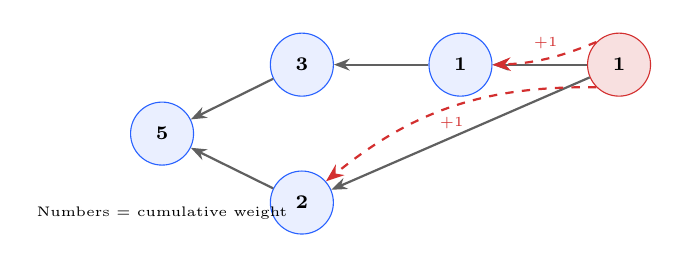
\begin{tikzpicture}[
      node distance=0.6cm and 1.2cm,
      tx/.style={circle, draw=tangleblue, fill=tangleblue!10, minimum size=0.8cm, font=\scriptsize},
      new/.style={circle, draw=tanglered, fill=tanglered!15, minimum size=0.8cm, font=\scriptsize},
      arr/.style={-{Stealth[length=2mm]}, thick, tanglegray}
    ]
      \node[tx] (G) {$\mathbf{5}$};
      \node[tx, above right=0.3cm and 1.2cm of G] (A) {$\mathbf{3}$};
      \node[tx, below right=0.3cm and 1.2cm of G] (B) {$\mathbf{2}$};
      \node[tx, right=1.2cm of A] (C) {$\mathbf{1}$};
      \node[new, right=1.2cm of C] (N) {\textbf{1}};

      \draw[arr] (A) -- (G);
      \draw[arr] (B) -- (G);
      \draw[arr] (C) -- (A);
      \draw[arr] (N) -- (C);
      \draw[arr] (N) -- (B);

      \draw[-{Stealth}, dashed, tanglered, thick] (N.south west) to[bend right=20] node[below, font=\tiny, tanglered] {+1} (B);
      \draw[-{Stealth}, dashed, tanglered, thick] (N.north west) to[bend left=10] node[above, font=\tiny, tanglered] {+1} (C);

      \node[below=0.4cm of G, font=\tiny] {Numbers = cumulative weight};
    \end{tikzpicture}
  \end{center}
\end{frame}

% ══════════════════════════════════════════════
\section{Tip Selection Algorithms}
% ══════════════════════════════════════════════

\begin{frame}{Overview of Tip Selection}
  \begin{block}{The Problem}
    When a new transaction is created, it must choose $m$ existing \textbf{tips} (unapproved transactions) to approve. The choice of tips directly affects:
    \begin{itemize}
      \item \textbf{Security} --- resistance to double-spend attacks
      \item \textbf{Liveness} --- all honest transactions eventually get confirmed
      \item \textbf{Tip pool size} $L(t)$ --- should remain bounded over time
    \end{itemize}
  \end{block}

  \vspace{0.3cm}
  \textbf{Three algorithms implemented:}
  \begin{enumerate}
    \item \textbf{Random Selection} --- uniform random from tip set
    \item \textbf{MCMC Selection} --- biased random walk with parameter $\alpha$
    \item \textbf{Hybrid Selection} --- two-phase: high-$\alpha$ (security) + low-$\alpha$ (liveness)
  \end{enumerate}
\end{frame}

\begin{frame}{Algorithm 1: Random Selection}
  \begin{block}{Procedure (Ferraro et al.\ \S IV-A)}
    Given tip set $\mathcal{T}$ and parameter $m$:
    \[
      \text{Select } m \text{ tips uniformly at random from } \mathcal{T}
    \]
  \end{block}

  \vspace{0.3cm}
  \textbf{Properties:}
  \begin{itemize}
    \item[\color{tangleteal}\checkmark] Simple and fast --- $O(m)$
    \item[\color{tangleteal}\checkmark] Fair --- every tip has equal chance
    \item[\color{tanglered}$\times$] \textbf{Vulnerable to attacks} --- does not prefer heavier (more trusted) branches
    \item[\color{tanglered}$\times$] No weight-based security guarantees
  \end{itemize}

  \vspace{0.3cm}
  \textbf{Class:} \texttt{RandomSelector} / \texttt{RandomTipSelector}
\end{frame}

\begin{frame}{Algorithm 2: MCMC Selection}
  \begin{block}{Biased Random Walk (Ferraro et al.\ \S II-A, Popov Whitepaper)}
    Starting from the \textbf{genesis}, walk forward through the DAG:
    \[
      P(\text{move to child } c_i) = \frac{\exp(\alpha \cdot \mathrm{CW}(c_i))}{\sum_j \exp(\alpha \cdot \mathrm{CW}(c_j))}
    \]
    Walk terminates when a \textbf{tip} (leaf node) is reached.
  \end{block}

  \vspace{0.3cm}
  \textbf{The role of $\alpha$:}
  \begin{itemize}
    \item $\alpha \to 0$: walk becomes \textbf{uniform} (equivalent to random)
    \item $\alpha$ large: walk \textbf{strongly prefers} branches with higher cumulative weight
    \item Trade-off: high $\alpha$ = more secure but may \textbf{orphan} low-weight tips
  \end{itemize}

  \vspace{0.2cm}
  \textbf{Class:} \texttt{MCMCSelector(alpha)} / \texttt{MCMCTipSelector(alpha)}
\end{frame}

\begin{frame}{Algorithm 3: Hybrid Selection (Main Contribution)}
  \begin{block}{Two-Phase Protocol (Ferraro, King \& Shorten \S III)}
    For each new transaction selecting $m$ parents:
    \begin{enumerate}
      \item \textbf{Security Step:} Select 1 tip via MCMC with \textbf{high} $\alpha_{\mathrm{high}}$
        \begin{itemize}
          \item Ensures attachment to the heaviest (most trusted) branch
          \item Provides double-spend resistance
        \end{itemize}
      \item \textbf{Swipe Step:} Select remaining $m-1$ tips via MCMC with \textbf{low} $\alpha_{\mathrm{low}}$
        \begin{itemize}
          \item Explores lighter branches, prevents orphaning
          \item Guarantees all tips are eventually approved
        \end{itemize}
    \end{enumerate}
  \end{block}

  \vspace{0.3cm}
  \textbf{Theoretical guarantee:} The tip pool size $L(t)$ remains \textbf{bounded} over time---every honest transaction is confirmed in finite time.

  \vspace{0.2cm}
  \textbf{Default parameters:} $\alpha_{\mathrm{high}} = 1.0$, $\alpha_{\mathrm{low}} = 0.001$

  \vspace{0.2cm}
  \textbf{Class:} \texttt{HybridSelector} / \texttt{HybridTipSelector}
\end{frame}

% ══════════════════════════════════════════════
\section{Distributed Architecture}
% ══════════════════════════════════════════════

\begin{frame}{Two Architectural Approaches}
  \begin{columns}[T]
    \begin{column}{0.48\textwidth}
      \begin{block}{\texttt{tangle-distributed}}
        \textbf{True multi-process:}
        \begin{itemize}
          \item Each node = separate OS process
          \item Spawned via \texttt{subprocess.Popen}
          \item Communication over \textbf{TCP sockets}
          \item Fully isolated memory
          \item More realistic model
        \end{itemize}
      \end{block}
    \end{column}
    \begin{column}{0.48\textwidth}
      \begin{block}{\texttt{tangle-sim}}
        \textbf{Single-process async:}
        \begin{itemize}
          \item Each node = \texttt{asyncio} task
          \item Managed by \texttt{SimulationEngine}
          \item Communication via \textbf{in-memory queues}
          \item Shared process memory
          \item Faster execution
        \end{itemize}
      \end{block}
    \end{column}
  \end{columns}

  \vspace{0.4cm}
  \begin{center}
    Both implementations share the same core algorithms, tip selection logic, and configuration format.
  \end{center}
\end{frame}

\begin{frame}{tangle-distributed: Process Architecture}
  \begin{center}
    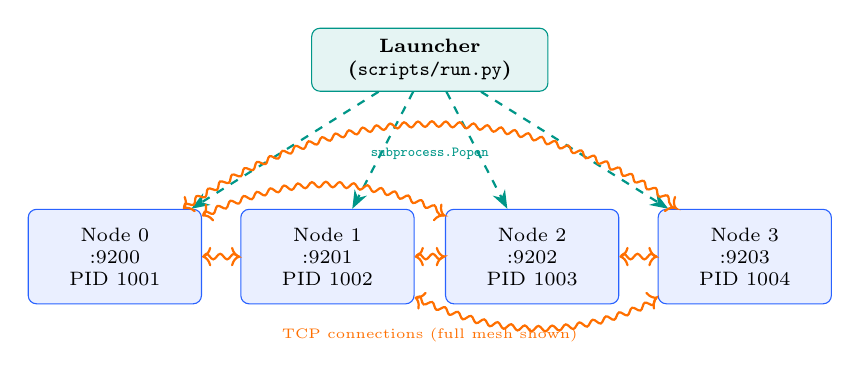
\begin{tikzpicture}[
      proc/.style={rectangle, draw=tangleblue, fill=tangleblue!10, rounded corners=3pt, minimum width=2.2cm, minimum height=1.2cm, align=center, font=\scriptsize},
      launcher/.style={rectangle, draw=tangleteal, fill=tangleteal!10, rounded corners=3pt, minimum width=3cm, minimum height=0.8cm, align=center, font=\scriptsize\bfseries},
      tcp/.style={<->, thick, tangleorange, decorate, decoration={snake, amplitude=1pt, segment length=5pt}},
      spawn/.style={-{Stealth}, thick, tangleteal, dashed}
    ]
      \node[launcher] (L) at (0, 2.5) {Launcher\\(\texttt{scripts/run.py})};

      \node[proc] (N0) at (-4, 0) {Node 0\\:9200\\PID 1001};
      \node[proc] (N1) at (-1.3, 0) {Node 1\\:9201\\PID 1002};
      \node[proc] (N2) at (1.3, 0) {Node 2\\:9202\\PID 1003};
      \node[proc] (N3) at (4, 0) {Node 3\\:9203\\PID 1004};

      \draw[spawn] (L) -- (N0);
      \draw[spawn] (L) -- (N1);
      \draw[spawn] (L) -- (N2);
      \draw[spawn] (L) -- (N3);

      \draw[tcp] (N0) -- (N1);
      \draw[tcp] (N1) -- (N2);
      \draw[tcp] (N2) -- (N3);
      \draw[tcp] (N0) to[bend left=25] (N2);
      \draw[tcp] (N1) to[bend right=25] (N3);
      \draw[tcp] (N0) to[bend left=35] (N3);

      \node[font=\tiny, tangleteal] at (0, 1.3) {\texttt{subprocess.Popen}};
      \node[font=\tiny, tangleorange] at (0, -1.0) {TCP connections (full mesh shown)};
    \end{tikzpicture}
  \end{center}
\end{frame}

\begin{frame}{Wire Protocol: Length-Prefixed JSON over TCP}
  \begin{block}{Frame Format}
    \begin{center}
      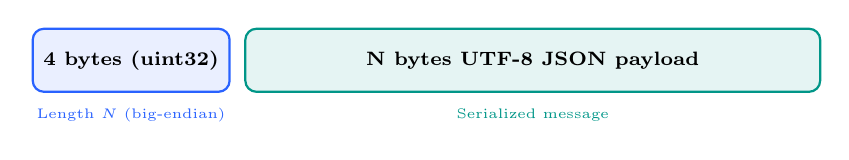
\begin{tikzpicture}
        \draw[thick, tangleblue, fill=tangleblue!10, rounded corners] (0,0) rectangle (2.5, 0.8);
        \draw[thick, tangleteal, fill=tangleteal!10, rounded corners] (2.7,0) rectangle (10, 0.8);
        \node[font=\scriptsize\bfseries] at (1.25, 0.4) {4 bytes (uint32)};
        \node[font=\scriptsize\bfseries] at (6.35, 0.4) {N bytes UTF-8 JSON payload};
        \node[font=\tiny, tangleblue] at (1.25, -0.3) {Length $N$ (big-endian)};
        \node[font=\tiny, tangleteal] at (6.35, -0.3) {Serialized message};
      \end{tikzpicture}
    \end{center}
  \end{block}

  \vspace{0.3cm}
  \textbf{Message Types:}
  \begin{columns}[T]
    \begin{column}{0.48\textwidth}
      \begin{itemize}
        \item \texttt{TX\_BROADCAST} --- gossip new transaction
        \item \texttt{TX\_REQUEST} --- request missing tx by ID
        \item \texttt{TX\_RESPONSE} --- reply with tx data
      \end{itemize}
    \end{column}
    \begin{column}{0.48\textwidth}
      \begin{itemize}
        \item \texttt{SYNC\_REQUEST} --- request full tangle
        \item \texttt{SYNC\_RESPONSE} --- send full tangle
        \item \texttt{PEER\_HELLO / \_ACK} --- handshake
      \end{itemize}
    \end{column}
  \end{columns}

  \vspace{0.3cm}
  \textbf{Gossip:} Flood-based with TTL field and deduplication by \texttt{msg\_id}.
\end{frame}

\begin{frame}{tangle-sim: Async Transport Architecture}
  \begin{center}
    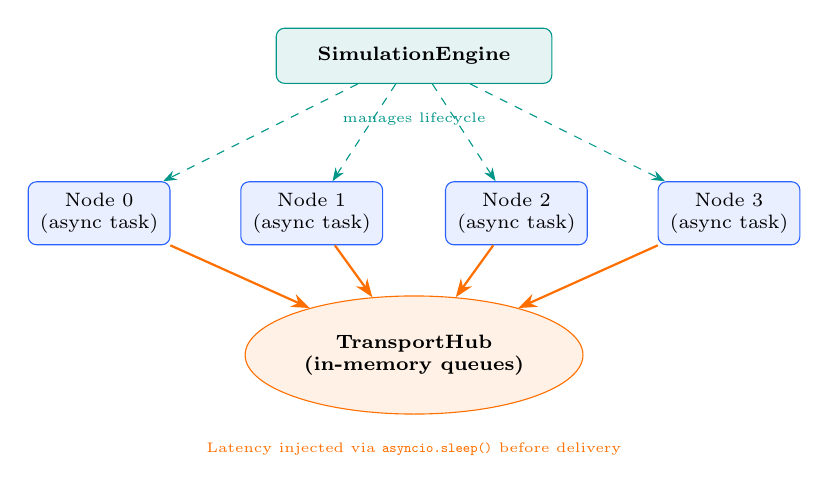
\begin{tikzpicture}[
      node distance=0.5cm,
      task/.style={rectangle, draw=tangleblue, fill=tangleblue!10, rounded corners=3pt, minimum width=1.8cm, minimum height=0.8cm, align=center, font=\scriptsize},
      hub/.style={ellipse, draw=tangleorange, fill=tangleorange!10, minimum width=3cm, minimum height=1.5cm, align=center, font=\scriptsize\bfseries},
      eng/.style={rectangle, draw=tangleteal, fill=tangleteal!10, rounded corners=3pt, minimum width=3.5cm, minimum height=0.7cm, align=center, font=\scriptsize\bfseries},
      qarr/.style={-{Stealth}, thick, tangleorange}
    ]
      \node[eng] (E) at (0, 3) {SimulationEngine};

      \node[task] (T0) at (-4, 1) {Node 0\\(async task)};
      \node[task] (T1) at (-1.3, 1) {Node 1\\(async task)};
      \node[task] (T2) at (1.3, 1) {Node 2\\(async task)};
      \node[task] (T3) at (4, 1) {Node 3\\(async task)};

      \node[hub] (H) at (0, -0.8) {TransportHub\\(in-memory queues)};

      \draw[qarr] (T0) -- (H);
      \draw[qarr] (T1) -- (H);
      \draw[qarr] (T2) -- (H);
      \draw[qarr] (T3) -- (H);

      \draw[-{Stealth}, dashed, tangleteal] (E) -- (T0);
      \draw[-{Stealth}, dashed, tangleteal] (E) -- (T1);
      \draw[-{Stealth}, dashed, tangleteal] (E) -- (T2);
      \draw[-{Stealth}, dashed, tangleteal] (E) -- (T3);

      \node[font=\tiny, tangleteal] at (0, 2.2) {manages lifecycle};
      \node[font=\tiny, tangleorange] at (0, -2.0) {Latency injected via \texttt{asyncio.sleep()} before delivery};
    \end{tikzpicture}
  \end{center}
\end{frame}

% ══════════════════════════════════════════════
\section{Message Passing \& Gossip}
% ══════════════════════════════════════════════

\begin{frame}{Gossip Protocol}
  \begin{columns}[T]
    \begin{column}{0.55\textwidth}
      \textbf{Flood-Based Gossip:}
      \begin{enumerate}
        \item Node creates or receives a new transaction
        \item Broadcasts \texttt{TX\_BROADCAST} to \textbf{all connected peers}
        \item Each peer checks \texttt{msg\_id} for deduplication
        \item If new: attach to local tangle, re-gossip to own peers
        \item TTL field decrements on each hop; message dies at TTL = 0
      \end{enumerate}

      \vspace{0.3cm}
      \textbf{Missing Parent Resolution:}
      \begin{itemize}
        \item If a received tx references unknown parents $\Rightarrow$ buffered in \texttt{\_pending}
        \item Periodic \texttt{TX\_REQUEST} sent for missing parent IDs
        \item On parent arrival: flush pending queue, attempt attachment
      \end{itemize}
    \end{column}
    \begin{column}{0.42\textwidth}
      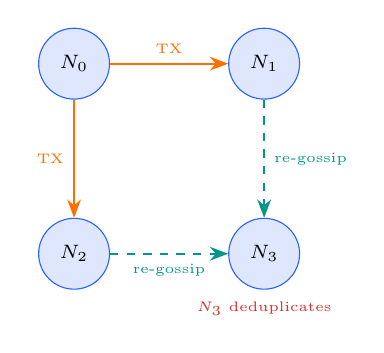
\begin{tikzpicture}[
        node distance=1.5cm,
        nd/.style={circle, draw=tangleblue, fill=tangleblue!15, minimum size=0.9cm, font=\scriptsize\bfseries},
        arr/.style={-{Stealth}, thick}
      ]
        \node[nd] (A) {$N_0$};
        \node[nd, right=1.5cm of A] (B) {$N_1$};
        \node[nd, below=1.5cm of A] (C) {$N_2$};
        \node[nd, below=1.5cm of B] (D) {$N_3$};

        \draw[arr, tangleorange] (A) -- node[above, font=\tiny] {TX} (B);
        \draw[arr, tangleorange] (A) -- node[left, font=\tiny] {TX} (C);
        \draw[arr, tangleteal, dashed] (B) -- node[right, font=\tiny] {re-gossip} (D);
        \draw[arr, tangleteal, dashed] (C) -- node[below, font=\tiny] {re-gossip} (D);

        \node[font=\tiny, tanglered] at ($(D) + (0, -0.7)$) {$N_3$ deduplicates};
      \end{tikzpicture}
    \end{column}
  \end{columns}
\end{frame}

\begin{frame}{Latency Model}
  \begin{block}{Simulated Network Latency}
    Every message delivery is delayed by a sampled latency value. Four models available:
  \end{block}

  \vspace{0.2cm}
  \begin{center}
    \begin{tabular}{lll}
      \toprule
      \textbf{Model} & \textbf{Sampling} & \textbf{Use Case} \\
      \midrule
      \texttt{constant} & $d = \text{base\_ms}$ & Baseline, debugging \\
      \texttt{uniform} & $d \sim U[\text{base} - j,\; \text{base} + j]$ & Simple jitter \\
      \texttt{normal} & $d \sim \mathcal{N}(\text{base},\; j^2)$ & Symmetric variation \\
      \texttt{lognormal} & $d \sim \text{LogNormal}(\mu, \sigma)$ & Realistic internet \\
      \bottomrule
    \end{tabular}
  \end{center}

  \vspace{0.3cm}
  \textbf{Implementation:}
  \begin{itemize}
    \item \texttt{tangle-distributed}: Delay injected \textbf{before TCP write} in \texttt{PeerConnection}
    \item \texttt{tangle-sim}: Delay via \texttt{asyncio.sleep()} in \texttt{TransportHub} before queue delivery
  \end{itemize}
\end{frame}

% ══════════════════════════════════════════════
\section{Network Topologies}
% ══════════════════════════════════════════════

\begin{frame}{Supported Network Topologies}
  \begin{center}
    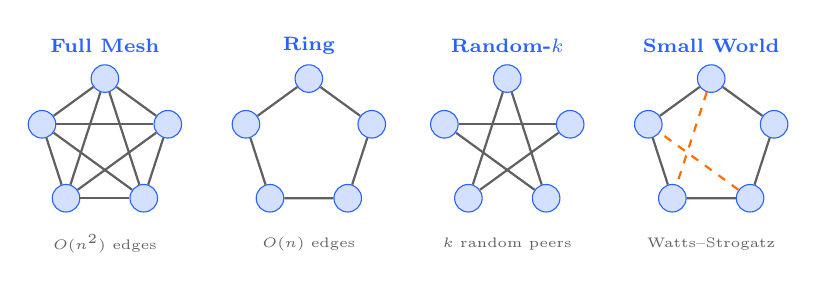
\begin{tikzpicture}[
      scale=0.7,
      nd/.style={circle, draw=tangleblue, fill=tangleblue!20, minimum size=0.35cm, inner sep=0pt},
      lnk/.style={thick, tanglegray}
    ]
      % Full Mesh
      \begin{scope}[shift={(-5.5, 0)}]
        \node[font=\scriptsize\bfseries, tangleblue] at (0, 1.8) {Full Mesh};
        \foreach \i in {1,...,5} {
          \node[nd] (fm\i) at ({90+72*(\i-1)}:1.2) {};
        }
        \foreach \i in {1,...,5} {
          \foreach \j in {\i,...,5} {
            \draw[lnk] (fm\i) -- (fm\j);
          }
        }
        \node[font=\tiny, tanglegray] at (0, -1.8) {$O(n^2)$ edges};
      \end{scope}

      % Ring
      \begin{scope}[shift={(-1.8, 0)}]
        \node[font=\scriptsize\bfseries, tangleblue] at (0, 1.8) {Ring};
        \foreach \i in {1,...,5} {
          \node[nd] (rg\i) at ({90+72*(\i-1)}:1.2) {};
        }
        \draw[lnk] (rg1)--(rg2)--(rg3)--(rg4)--(rg5)--(rg1);
        \node[font=\tiny, tanglegray] at (0, -1.8) {$O(n)$ edges};
      \end{scope}

      % Random-k
      \begin{scope}[shift={(1.8, 0)}]
        \node[font=\scriptsize\bfseries, tangleblue] at (0, 1.8) {Random-$k$};
        \foreach \i in {1,...,5} {
          \node[nd] (rk\i) at ({90+72*(\i-1)}:1.2) {};
        }
        \draw[lnk] (rk1)--(rk3);
        \draw[lnk] (rk1)--(rk4);
        \draw[lnk] (rk2)--(rk5);
        \draw[lnk] (rk2)--(rk4);
        \draw[lnk] (rk3)--(rk5);
        \node[font=\tiny, tanglegray] at (0, -1.8) {$k$ random peers};
      \end{scope}

      % Small World
      \begin{scope}[shift={(5.5, 0)}]
        \node[font=\scriptsize\bfseries, tangleblue] at (0, 1.8) {Small World};
        \foreach \i in {1,...,5} {
          \node[nd] (sw\i) at ({90+72*(\i-1)}:1.2) {};
        }
        \draw[lnk] (sw1)--(sw2)--(sw3)--(sw4)--(sw5)--(sw1);
        \draw[lnk, tangleorange, dashed] (sw1)--(sw3);
        \draw[lnk, tangleorange, dashed] (sw4)--(sw2);
        \node[font=\tiny, tanglegray] at (0, -1.8) {Watts--Strogatz};
      \end{scope}
    \end{tikzpicture}
  \end{center}

  \vspace{0.2cm}
  Also supports: \textbf{Star} topology (hub-spoke).

  \vspace{0.2cm}
  \textbf{Note:} \texttt{tangle-distributed} builds an adjacency list from the topology and distributes peer lists to each node config. \texttt{tangle-sim} uses \texttt{NetworkTopology} class with factory methods.
\end{frame}

% ══════════════════════════════════════════════
\section{Node Lifecycle}
% ══════════════════════════════════════════════

\begin{frame}{Node Lifecycle (tangle-distributed)}
  \begin{center}
    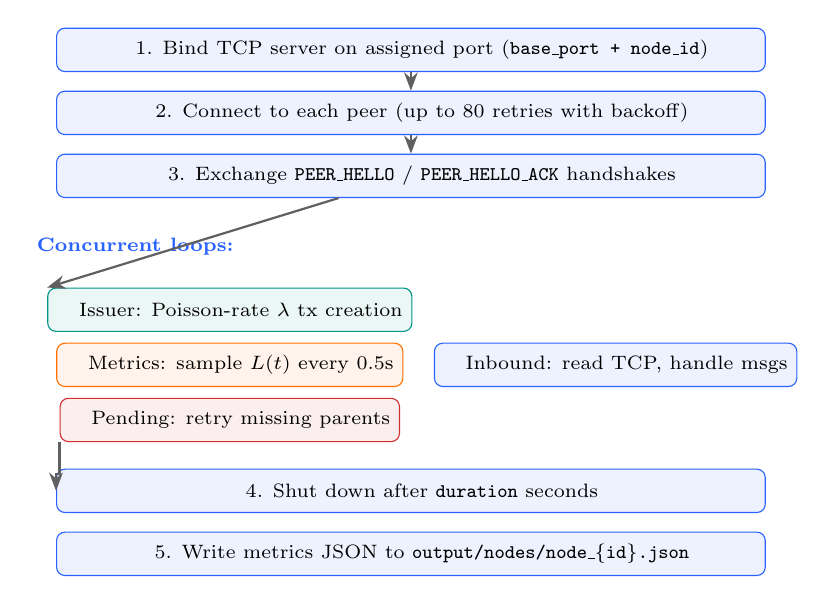
\begin{tikzpicture}[
      node distance=0.6cm,
      phase/.style={rectangle, draw=tangleblue, fill=tangleblue!8, rounded corners=3pt, minimum width=9cm, minimum height=0.55cm, font=\scriptsize, align=left},
      label/.style={font=\scriptsize\bfseries, tangleblue},
      arr/.style={-{Stealth}, thick, tanglegray}
    ]
      \node[phase] (P1) at (0, 4) {\quad 1. Bind TCP server on assigned port (\texttt{base\_port + node\_id})};
      \node[phase] (P2) at (0, 3.2) {\quad 2. Connect to each peer (up to 80 retries with backoff)};
      \node[phase] (P3) at (0, 2.4) {\quad 3. Exchange \texttt{PEER\_HELLO} / \texttt{PEER\_HELLO\_ACK} handshakes};

      \node[label] at (-3.5, 1.5) {Concurrent loops:};

      \node[phase, fill=tangleteal!8, draw=tangleteal, minimum width=4.2cm] (L1) at (-2.3, 0.7) {\quad Issuer: Poisson-rate $\lambda$ tx creation};
      \node[phase, fill=tangleorange!8, draw=tangleorange, minimum width=4.2cm] (L2) at (-2.3, 0.0) {\quad Metrics: sample $L(t)$ every 0.5s};
      \node[phase, fill=tanglered!8, draw=tanglered, minimum width=4.2cm] (L3) at (-2.3, -0.7) {\quad Pending: retry missing parents};
      \node[phase, fill=tangleblue!8, draw=tangleblue, minimum width=4.2cm] (L4) at (2.6, 0.0) {\quad Inbound: read TCP, handle msgs};

      \node[phase] (P4) at (0, -1.6) {\quad 4. Shut down after \texttt{duration} seconds};
      \node[phase] (P5) at (0, -2.4) {\quad 5. Write metrics JSON to \texttt{output/nodes/node\_\{id\}.json}};

      \draw[arr] (P1) -- (P2);
      \draw[arr] (P2) -- (P3);
      \draw[arr] (P3) -- (L1.north west);
      \draw[arr] (L3.south west) -- ++(0, -0.4) -| (P4.west);
    \end{tikzpicture}
  \end{center}
\end{frame}

\begin{frame}{Transaction Issuance Flow}
  \begin{center}
    \begin{tikzpicture}[
      node distance=0.5cm and 1cm,
      step/.style={rectangle, draw=tangleblue, fill=tangleblue!8, rounded corners=3pt, minimum width=2.6cm, minimum height=0.7cm, font=\scriptsize, align=center},
      arr/.style={-{Stealth}, thick, tanglegray}
    ]
      \node[step] (S1) at (0, 0) {Wait for\\Poisson interval};
      \node[step] (S2) at (3.2, 0) {Select $m$ tips\\(tip selector)};
      \node[step] (S3) at (6.4, 0) {Create TX\\(random value)};
      \node[step] (S4) at (9.6, 0) {Simulate PoW\\(\texttt{asyncio.sleep(h)})};
      \node[step] (S5) at (4.8, -1.5) {Attach to\\local tangle};
      \node[step] (S6) at (8, -1.5) {Broadcast via\\gossip protocol};

      \draw[arr] (S1) -- (S2);
      \draw[arr] (S2) -- (S3);
      \draw[arr] (S3) -- (S4);
      \draw[arr] (S4) |- (S5);
      \draw[arr] (S5) -- (S6);
    \end{tikzpicture}
  \end{center}

  \vspace{0.3cm}
  \textbf{Poisson process:} Inter-arrival time $\sim \mathrm{Exp}(1/\lambda)$, where $\lambda$ = \texttt{tx\_rate} per node.

  \vspace{0.2cm}
  \textbf{Proof of Work:} Simulated as an \texttt{asyncio.sleep(h)} delay (configurable $h$ seconds). Transaction status transitions: \textsc{Pending\_PoW} $\to$ \textsc{Attached}.
\end{frame}

% ══════════════════════════════════════════════
\section{Validation \& Security}
% ══════════════════════════════════════════════

\begin{frame}{Validation \& Double-Spend Detection}
  \begin{columns}[T]
    \begin{column}{0.55\textwidth}
      \textbf{Double-Spend Detection:}
      \begin{itemize}
        \item Checks if two transactions from the same \texttt{sender\_addr} spend conflicting values
        \item Uses \texttt{approval\_path()} to detect conflicting branches
        \item Transactions on conflicting branches are flagged
      \end{itemize}

      \vspace{0.3cm}
      \textbf{Consistency Checking} (\texttt{tangle-sim}):
      \begin{itemize}
        \item \texttt{ConsistencyChecker} validates DAG invariants:
          \begin{itemize}
            \item All parents exist in the tangle
            \item No orphaned references
            \item Genesis is reachable from every tx
          \end{itemize}
      \end{itemize}
    \end{column}
    \begin{column}{0.42\textwidth}
      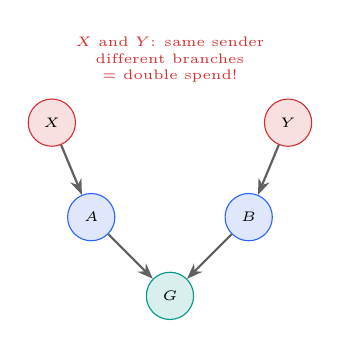
\begin{tikzpicture}[
        tx/.style={circle, draw=tangleblue, fill=tangleblue!15, minimum size=0.6cm, font=\tiny\bfseries},
        bad/.style={circle, draw=tanglered, fill=tanglered!15, minimum size=0.6cm, font=\tiny\bfseries},
        gen/.style={circle, draw=tangleteal, fill=tangleteal!15, minimum size=0.6cm, font=\tiny\bfseries},
        arr/.style={-{Stealth[length=2mm]}, thick, tanglegray}
      ]
        \node[gen] (G) at (0,0) {$G$};
        \node[tx] (A) at (-1, 1) {$A$};
        \node[tx] (B) at (1, 1) {$B$};
        \node[bad] (X) at (-1.5, 2.2) {$X$};
        \node[bad] (Y) at (1.5, 2.2) {$Y$};

        \draw[arr] (A) -- (G);
        \draw[arr] (B) -- (G);
        \draw[arr] (X) -- (A);
        \draw[arr] (Y) -- (B);

        \node[font=\tiny, tanglered, align=center] at (0, 3) {$X$ and $Y$: same sender\\different branches\\= double spend!};
      \end{tikzpicture}
    \end{column}
  \end{columns}
\end{frame}

% ══════════════════════════════════════════════
\section{Configuration \& Scenarios}
% ══════════════════════════════════════════════

\begin{frame}{Configuration System}
  \textbf{YAML-based hierarchical configuration:}

  \vspace{0.2cm}
  \begin{columns}[T]
    \begin{column}{0.48\textwidth}
      \textbf{Key Parameters:}
      \vspace{0.1cm}

      \begin{tabular}{lll}
        \toprule
        \textbf{Param} & \textbf{Symbol} & \textbf{Meaning} \\
        \midrule
        \texttt{tx\_rate} & $\lambda$ & Poisson rate/node \\
        \texttt{alpha} & $\alpha$ & MCMC bias \\
        \texttt{alpha\_high} & $\alpha_H$ & Hybrid security \\
        \texttt{alpha\_low} & $\alpha_L$ & Hybrid swipe \\
        \texttt{pow.h} & $h$ & PoW delay (sec) \\
        \texttt{m} & $m$ & Parents per tx \\
        \texttt{duration} & $T$ & Sim length (sec) \\
        \bottomrule
      \end{tabular}
    \end{column}
    \begin{column}{0.48\textwidth}
      \textbf{Predefined Scenarios:}
      \begin{itemize}
        \item \texttt{small\_network}: 3 nodes, 15s, full mesh, uniform latency
        \item \texttt{large\_network}: 8 nodes, 45s, small-world, lognormal latency
        \item \texttt{attack\_scenario}: 7 nodes, one attacker at $4\times$ rate
        \item \texttt{mcmc\_comparison}: Pure MCMC study, $\alpha = 0.01$
      \end{itemize}

      \vspace{0.2cm}
      Supports \textbf{per-node overrides} (e.g., attacker with custom $\lambda$).
    \end{column}
  \end{columns}
\end{frame}

% ══════════════════════════════════════════════
\section{Simulation Flow \& Metrics}
% ══════════════════════════════════════════════

\begin{frame}{End-to-End Simulation Flow}
  \begin{center}
    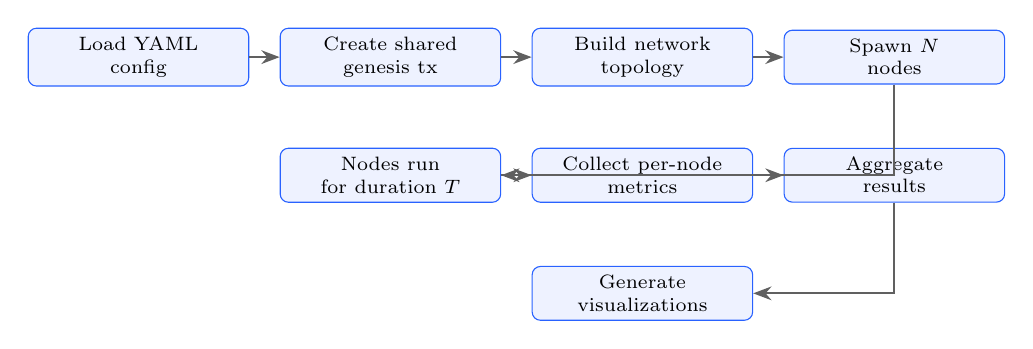
\begin{tikzpicture}[
      box/.style={rectangle, draw=tangleblue, fill=tangleblue!8, rounded corners=3pt, minimum width=2.8cm, minimum height=0.6cm, font=\scriptsize, align=center},
      arr/.style={-{Stealth}, thick, tanglegray}
    ]
      \node[box] (C) at (0, 0) {Load YAML\\config};
      \node[box] (G) at (3.2, 0) {Create shared\\genesis tx};
      \node[box] (T) at (6.4, 0) {Build network\\topology};
      \node[box] (S) at (9.6, 0) {Spawn $N$\\nodes};
      \node[box] (R) at (3.2, -1.5) {Nodes run\\for duration $T$};
      \node[box] (M) at (6.4, -1.5) {Collect per-node\\metrics};
      \node[box] (A) at (9.6, -1.5) {Aggregate\\results};
      \node[box] (V) at (6.4, -3) {Generate\\visualizations};

      \draw[arr] (C) -- (G);
      \draw[arr] (G) -- (T);
      \draw[arr] (T) -- (S);
      \draw[arr] (S) |- (R);
      \draw[arr] (R) -- (M);
      \draw[arr] (M) -- (A);
      \draw[arr] (A) |- (V);
    \end{tikzpicture}
  \end{center}
\end{frame}

\begin{frame}{Metrics \& Outputs}
  \textbf{Per-Node Metrics:}
  \begin{itemize}
    \item \texttt{tip\_history}: $L(t)$ time series --- tip count sampled every 0.5s
    \item \texttt{issued} / \texttt{received}: transaction logs with timestamps
    \item \texttt{latencies}: propagation delay measurements (ms)
    \item \texttt{edges}: DAG edge list for visualization
  \end{itemize}

  \vspace{0.3cm}
  \textbf{Aggregated Metrics:}
  \begin{itemize}
    \item \textbf{Convergence ratio} = $\frac{|\bigcap_i T_i|}{|\bigcup_i T_i|}$ \quad (intersection / union of all tangles)
    \item \textbf{Orphan rate} = $\frac{\text{avg final tips}}{\text{avg tangle size}}$
    \item \textbf{Average propagation latency} across all transactions
    \item \textbf{Total unique transactions} across all nodes
  \end{itemize}

  \vspace{0.3cm}
  \textbf{Visualization Dashboard} (6 panels): $L(t)$ curves, tangle sizes, latency histogram, cumulative weight distribution, throughput, convergence heatmap.
\end{frame}

% ══════════════════════════════════════════════
\section{Comparison of Implementations}
% ══════════════════════════════════════════════

\begin{frame}{tangle-distributed vs.\ tangle-sim}
  \begin{center}
    \small
    \begin{tabular}{lcc}
      \toprule
      \textbf{Aspect} & \textbf{tangle-distributed} & \textbf{tangle-sim} \\
      \midrule
      Process model & Separate OS processes & Single process, async tasks \\
      IPC mechanism & Raw TCP sockets & In-memory queues \\
      Wire format & Length-prefixed JSON & Python objects \\
      Memory isolation & Fully isolated & Shared memory \\
      Latency injection & Before TCP write & \texttt{asyncio.sleep()} \\
      Network library & Pure \texttt{asyncio} + stdlib & Optional ZMQ \\
      Graph library & Manual adjacency & \texttt{networkx} \\
      Realism & Higher & Lower \\
      Speed & Slower (IPC overhead) & Faster \\
      Scale tested & Up to 8 nodes & Up to 10 nodes \\
      \bottomrule
    \end{tabular}
  \end{center}
\end{frame}

% ══════════════════════════════════════════════
\section{Summary}
% ══════════════════════════════════════════════

\begin{frame}{Summary}
  \begin{enumerate}
    \item \textbf{DAG-based ledger}: Transactions form a directed acyclic graph (Tangle) where each new transaction approves $m$ existing tips
    \item \textbf{Three tip selection algorithms}: Random, MCMC (parameterized by $\alpha$), and Hybrid (two-phase: security + swipe)
    \item \textbf{Hybrid guarantees}: Bounded $L(t)$ and eventual confirmation of all honest transactions
    \item \textbf{Two implementations}: Multi-process TCP (realistic) and single-process async (fast)
    \item \textbf{Configurable simulation}: YAML-driven scenarios with tunable topology, latency, attack models, and algorithm parameters
    \item \textbf{Rich metrics}: Convergence, orphan rates, propagation latency, and visual dashboards
  \end{enumerate}

  \vspace{0.3cm}
  \begin{block}{References}
    \small
    \begin{itemize}
      \item \v{Z}ivi\'{c} et al., ``DAG as Tangle,'' TELFOR 2019
      \item Ferraro, King \& Shorten, ``Stability of Unverified Transactions,'' IEEE 2020
      \item Popov, ``The Tangle,'' IOTA Whitepaper, 2018
    \end{itemize}
  \end{block}
\end{frame}

\begin{frame}{}
  \begin{center}
    {\Huge\bfseries Thank You}

    \vspace{1cm}
    {\large Questions?}
  \end{center}
\end{frame}

\end{document}
